\documentclass[]{beamer}
\usepackage[utf8]{inputenc}
\usetheme{Madrid}
\usepackage{fancyvrb}
\usepackage{etoolbox}
\usepackage{tikz}
\usepackage[compat=1.1.0]{tikz-feynman}
\usepackage{ifluatex}

%
% COLOR TEMPLATE
%
\definecolor{vandy_gold}{RGB}{204, 161, 102}
\definecolor{vandy_blue}{RGB}{18, 111, 150}
\definecolor{vandy_red}{RGB}{153, 61, 27}
\definecolor{vandy_gray}{RGB}{51, 51, 51}
\definecolor{vandy_green}{RGB}{70, 78, 33}

\setbeamercolor{section in toc}{fg=vandy_gold,bg=white}
\setbeamercolor{alerted text}{fg=vandy_red}
\setbeamercolor*{palette primary}{fg=white,bg=black}
\setbeamercolor*{palette secondary}{fg=white,bg=vandy_gold}
\setbeamercolor*{palette tertiary}{fg=white,bg=black}
\setbeamercolor*{palette quaternary}{fg=white,bg=vandy_gold}
\setbeamercolor*{sidebar}{fg=white,bg=black}
\setbeamercolor*{palette sidebar primary}{fg=white}
\setbeamercolor*{palette sidebar secondary}{fg=white}
\setbeamercolor*{palette sidebar tertiary}{fg=white}
\setbeamercolor*{palette sidebar quaternary}{fg=white}
\setbeamercolor{titlelike}{parent=palette secondary}
\setbeamercolor{frametitle}{fg=white,bg=vandy_gold}
\setbeamercolor{frametitle right}{fg=white,bg=vandy_gold}
\setbeamercolor{section number projected}{bg=black,fg=vandy_gold}
\setbeamercolor{section in toc}{fg=black}
\setbeamercolor{block title}{fg=white, bg=vandy_gray!50!white}
\setbeamercolor{block body}{bg=vandy_gray!20!white}

%
% BEAMER SETTINGS
%
\setbeamertemplate{itemize item}{\color{black}$\bullet$}
\setbeamerfont{block title}{size=\small}
\setbeamerfont{block body}{size=\tiny}
\AtBeginEnvironment{tabular}{\tiny}
\tikzset{font=\tiny}
%\includeonlyframes{current}

%
% TITLE SLIDE INFO
%
\title[VBF Axion DM Search]{Axion DM Search with Vector Boson Fusion}
\author[E. Sheridan]{A. Gurrola\inst{1}, \textbf{E. Sheridan}\inst{1}, B. Soubasis\inst{1}}
\institute{Vanderbilt University\inst{1}}



%			              %
%                         %
%  DOCUMENT               %
%                         %
%                         %
\begin{document}

% 1) TITLE PAGE
\frame{\titlepage}

% 2) TABLE OF CONTENTS
\begin{frame}{Table of Contents}
\tableofcontents
\end{frame}



%
% SEC: PROJECT INTRODUCTION
%
\section{Project Introduction}

% 3) MOTIVATING AXIONS
\begin{frame}{Motivating Axions}
    \begin{block}<+(1)->{Theoretical Origins}
        \begin{itemize}
            \item The structure of quantum chromodynamics permits a violation of the combined charge conjugation-parity symmetry, but experimental constraints (stemming from symmetry breaking repercussions on the neutron electric dipole moment) require this violation to be small
            \item It is unclear why this symmetry violation should simultaneously exist and be so small: this is the \textbf{strong CP problem}
            \item Roberto Peccei and Helen Quinn addressed this conundrum in 1977 by promoting the CP violation phase $\overline{\Theta}$---previously a Standard Model input requiring experimental measurement---to a scalar field which spontaneously breaks a new global symmetry (a Peccei–Quinn symmetry)
            \item The quanta (or boson) of this new scalar field is the \textbf{axion}
        \end{itemize}
    \end{block}
    
    \smallskip
    
    \begin{block}<+(1)->{Axion Properties}
        \begin{itemize}
            \item The axion is a neutral spin-$0$ boson, and different models permit widely varied mass values
            \item If the axion is sufficiently light, it presents itself as a dark matter candidate particle
            \item Axion theories require minor modifications to classical electrodynamics, as the presence of the axion serves to ``rotate'' the electric and magnetic fields into each other to an extent proportional to axion coupling and field strength 
        \end{itemize}
    \end{block}
    
    \smallskip
    
    \begin{block}<+(1)->{Axion Literature}
        \begin{itemize}
            \item Astrophysics/cosmological experiments place bounds on axions and axion-like particles (ALPs) masses in some models, requiring them to be eV scale or lighter
            \item However, there still exist models which enable axions and ALPs to have masses in the MeV and GeV scales
            \item ``Heavy axions'' have been studied at the LHC, but primarily at higher mass scales due to sensitivity limitations  
        \end{itemize}
    \end{block}
\end{frame}

% 4) MOTIVATING VBF
\begin{frame}{Motivating the Vector Boson Fusion Approach}
    \centering
    \uncover<+(1)->{
        \scalebox{0.8}{
            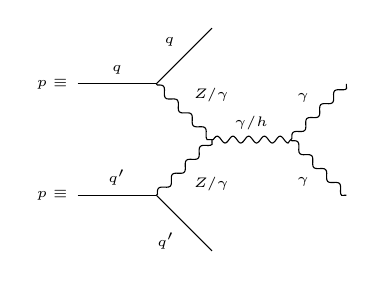
\begin{tikzpicture}
                \begin{feynman}[small]
                    % top to bottom, pre-axion
                    \vertex (v1); % top jet vertex
                    \vertex [left=of v1] (in1) {$p \equiv$}; % top incoming particle
                    \vertex [above right=of v1] (j1) ; % top jet
                    \vertex [below right=of v1] (v3); % axion vertex
                    \vertex [below left=of v3] (v2); % bottom jet vertex
                    \vertex [below right=of v2] (j2);  % bottom jet
                    \vertex [left=of v2] (in2) {$p \equiv $};  % bottom incoming particle
                    % axion onward
                    \vertex [right=of v3] (ax);
                    \vertex [above right=of ax] (p1);
                    \vertex [below right=of ax] (p2);
                    
                    \diagram*{
                        (in1) -- [plain, edge label=$q$] (v1),
                        (in2) -- [plain, edge label=$q'$] (v2),
                        (v1) -- [plain, edge label=$q$] (j1),
                        (v2) -- [plain, edge label'=$q'$] (j2),
                        (v1) -- [boson, edge label=$Z/\gamma$] (v3),
                        (v2) -- [boson, edge label'=$Z/\gamma$] (v3),
                        (v3) -- [boson, edge label=$\gamma/h$] (ax),
                        (ax) -- [boson, edge label=$\gamma$] (p1),
                        (ax) -- [boson, edge label'=$\gamma$] (p2),
                    };
                \end{feynman}
            \end{tikzpicture}
        }
    }
    
    \begin{block}<+(1)->{Description}
        \begin{itemize}
            \item Vector boson fusion processes (VBF; exhibited above) are experimentally important due to their distinctiveness at the LHC
            \item In particular, the so-called ``tagged jets'' (the outgoing quarks in the above diagram) carry tell-tale high pseudorapidities
            \item This VBF kinematic signature suppresses background
            \item VBF cross sections typically surpass those of other topologies (Drell-Yan, etc) in new-physics processes with heavy new particles
        \end{itemize}
    \end{block}
\end{frame}



%
% SAMPLES AND SIMULATION
%
\section{Samples and Simulation}

% 5) SIGNAL GENERATION
\begin{frame}{Signal Generation}
    \begin{center}
        \begin{block}<+(1)->{Process}
            Signal generated using \textbf{MadGraph} (version \textbf{2.6.5}).
            
            \smallskip
            
            \texttt{import model ALP\_chiral\_UFO} \newline
            \texttt{generate p p > ax j j QCD=0, ax > a a}
            
            \smallskip
            
            We choose to consider an axion mass of \textbf{1 MeV}. Only default MadGraph cuts employed: e.g., $p_T^j > 20$ GeV, $p_T^\gamma > 10$ GeV
        \end{block}
        
    \uncover<+(1)->{
        \scalebox{0.75}{
            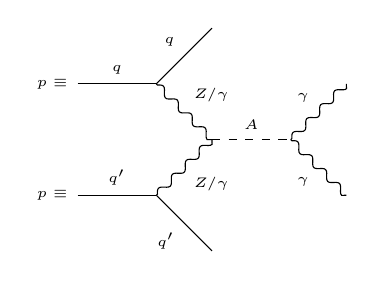
\begin{tikzpicture}
                \begin{feynman}[small]
                    % top to bottom, pre-axion
                    \vertex (v1); % top jet vertex
                    \vertex [left=of v1] (in1) {$p \equiv$}; % top incoming particle
                    \vertex [above right=of v1] (j1) ; % top jet
                    \vertex [below right=of v1] (v3); % axion vertex
                    \vertex [below left=of v3] (v2); % bottom jet vertex
                    \vertex [below right=of v2] (j2);  % bottom jet
                    \vertex [left=of v2] (in2) {$p \equiv $};  % bottom incoming particle
                    % axion onward
                    \vertex [right=of v3] (ax);
                    \vertex [above right=of ax] (p1);
                    \vertex [below right=of ax] (p2);
                    
                    \diagram*{
                        (in1) -- [plain, edge label=$q$] (v1),
                        (in2) -- [plain, edge label=$q'$] (v2),
                        (v1) -- [plain, edge label=$q$] (j1),
                        (v2) -- [plain, edge label'=$q'$] (j2),
                        (v1) -- [boson, edge label=$Z/\gamma$] (v3),
                        (v2) -- [boson, edge label'=$Z/\gamma$] (v3),
                        (v3) -- [scalar, edge label=$A$] (ax),
                        (ax) -- [boson, edge label=$\gamma$] (p1),
                        (ax) -- [boson, edge label'=$\gamma$] (p2),
                    };
                \end{feynman}
            \end{tikzpicture}
        }
    }
            
    \begin{block}<+(1)->{Comments}
        \begin{itemize}
            \item \texttt{QCD = 0} selected due to our interest in axions with \textbf{negligible strong force couplings}
            \item \texttt{ax > a a} channel selected due to our emphasis on \textbf{lighter axions} (photons dominating heavier bosons)
            \item The significance of our studies arises in part from small axion mass scales probed
        \end{itemize}
    \end{block}
        
    \end{center}
\end{frame}

% 6) INITIAL KINEMATICS
\begin{frame}{Initial Kinematics}
    \begin{columns}
        \begin{column}{0.45\linewidth}
            \centering
            \includegraphics<+(1)->[width=0.8\linewidth]{images/no_mg_cuts_kinematics/selection_8.png} % delta eta jj\\
            
            \bigskip
            
            \includegraphics<+(1)->[width=0.8\linewidth]{images/no_mg_cuts_kinematics/selection_7.png} % m jj
        \end{column}
        \begin{column}{0.5\linewidth}
            \begin{block}<+(1)->{Comments}
                \begin{itemize}
                    \item Total cross section for signal is $0.786 \pm 0.001$ pb
                    \item VBF processes are characterized by high $|\Delta \eta^{jj}|$, so a peak at $0$ indicates that other processes dominate
                    \item An $m^{jj}$ peak at approx. $80$-$90$ GeV indicates dominating \texttt{Z/W+/W- > j j} processes
                    
                    \smallskip
                    
                    \begin{tabular}{|c|c|}
                        \hline
                        Channel & Cross-Section (pb) \\
                        \hline
                        \hline
                        \texttt{g g > ax g g} & $0.731 \pm 1\text{e-}3$\\
                        \texttt{u d > ax u d} & $0.02414 \pm 2\text{e-}4$\\
                        \texttt{u u > ax u u} & $0.01549 \pm 6\text{e-}5$\\
                        \hline
                    \end{tabular}
                    
                    \smallskip
                    
                    \item Channel with next highest cross section on order of $1$ fb.
                    \item \texttt{q q > ax q q} processes can take on a VBF topology, but the \texttt{g g > ax g g} channel does not
                    \item Despite the higher cross section, we avoid gluon-gluon processes due to their extensive prior analysis in the axion conext
                    \item Additionally, gluon-gluon approaches are insensitive to light axions
                \end{itemize}
            \end{block}
        \end{column}
    \end{columns}
\end{frame}

% 7) VBF PURITY
\begin{frame}{Increasing VBF Purity in Signal}
    \begin{columns}
        \begin{column}{0.45\linewidth}
            \begin{block}<+(1)->{Objective}
                \begin{itemize}
                    \item Want to generate signal events in a phase space region which emphasizes our eventual optimization (ensuring sufficient statistics)
                    \item Equivalently, want to generate signal events primarily with the particular topologies (VBF) we will later select
                    \item Thus before comparing with background, want to impose \textbf{MadGraph-level cuts} on signal events
                    \item We select two topologies to try and minimize with such cuts: \texttt{g g > ax g g} and \texttt{Z > j j}
                \end{itemize}
            \end{block}
            
            \smallskip
            
            \centering
            \uncover<+(1)->{
                \scalebox{0.6}{
                    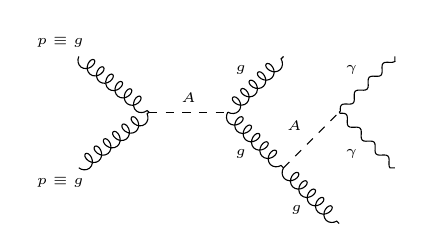
\begin{tikzpicture}
                        \begin{feynman}[small]
                            \vertex  (v1); % gluon-gluon vertex
                            \vertex [above left=of v1] (g1) {$p \equiv g$}; % top incoming gluon
                            \vertex [below left=of v1] (g2) {$p \equiv g$}; % bottom incoming gluon
                            \vertex [right=of v1] (ax1); % first axion vertex
                            \vertex [above right=of ax1] (g3); % top outgoing gluon
                            \vertex [below right=of ax1] (v2); % gluon decay vertex
                            \vertex [above right=of v2] (ax2); % second (final) axion vertex
                            \vertex [above right=of ax2] (p1); % top photon
                            \vertex [below right=of ax2] (p2); % bottom photon
                            \vertex [below right=of v2] (g4); % bottom outgoing gluon
                            
                            \diagram*{
                                (g1) -- [gluon] (v1),
                                (g2) -- [gluon] (v1),
                                (v1) -- [scalar, edge label=$A$] (ax1),
                                (ax1) -- [gluon, edge label=$g$] (g3),
                                (ax1) -- [gluon, edge label'=$g$] (v2),
                                (v2) -- [scalar, edge label=$A$] (ax2),
                                (v2) -- [gluon, edge label'=$g$] (g4),
                                (ax2) -- [boson, edge label=$\gamma$] (p1),
                                (ax2) -- [boson, edge label'=$\gamma$] (p2),
                            };
                        \end{feynman}
                    \end{tikzpicture}
                }
            }
            
            \smallskip
            
            \uncover<+(1)->{
                \scalebox{0.6}{
                    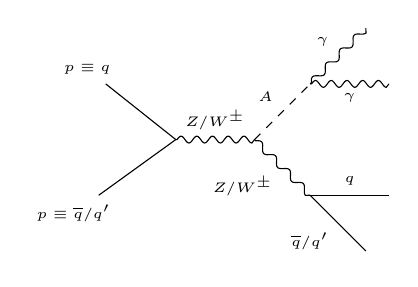
\begin{tikzpicture}
                        \begin{feynman}[small]
                            \vertex (v1);
                            \vertex [above left=of v1] (in1) {$p \equiv q$}; % top incoming particle
                            \vertex [below left=of v1] (in2) {$p \equiv \overline{q} / q'$}; % bottom incoming particle
                            \vertex [right=of v1] (ax1); % first axion vertex
                            \vertex [above right=of ax1] (ax2); % second axion
                            \vertex [above right=of ax2] (p1); % top photon
                            \vertex [right=of ax2] (p2); % bottom photon
                            \vertex [below right=of ax1] (v2); % z boson decay vertex
                            \vertex [right=of v2] (j1); % top outgoing jet
                            \vertex [below right=of v2] (j2); % bottom outgoing jet
                            
                            
                            \diagram*{
                                (in1) -- [plain] (v1),
                                (in2) -- [plain] (v1),
                                (v1) -- [boson, edge label=$Z/W^\pm$] (ax1),
                                (ax1) -- [scalar, edge label=$A$] (ax2),
                                (ax1) -- [boson, edge label'=$Z/W^\pm$] (v2),
                                (v2) -- [plain, edge label=$q$] (j1),
                                (v2) -- [plain, edge label'=$\overline{q} / q'$] (j2),
                                (ax2) -- [boson, edge label=$\gamma$] (p1),
                                (ax2) -- [boson, edge label'=$\gamma$] (p2),
                            };
                        \end{feynman}
                    \end{tikzpicture}
                }
            }
        \end{column}
        \begin{column}{0.45\linewidth}
            \begin{block}<+(1)->{Final Approach}
                Choose to generate $1000000$ signal events with all of the previous commands/setting, along with the following additional MadGraph selections. \newline
                $|\Delta \eta^{jj}| > 2.4$, $m^{jj} > 120$ GeV
                \begin{itemize}
                    \item The gluon-gluon channel exhibits predominately low $|\Delta \eta^{jj}|$, so we apply a cut with the hopes of reducing its cross section
                    \item The vector boson resonance channel satisfies $m^{jj} \approx 80$ GeV, so we apply an $m^{jj}$ cut with the hopes of also reducing that cross section
                \end{itemize}
                The cross section for this signal is $0.10235 \pm 2.82\text{e-}5$ pb, and the following breakdown of individual channel cross-sections gives a first indication of our success. While the gluon-gluon channel still dominates, we've achieved a VBF signal purity sufficient to achieve the necessary statistics during optimization.
            \end{block}
            
            \bigskip
            
            \centering
            \uncover<+(1)->{
                \begin{tabular}{|c|c|}
                    \hline
                    Channel & Cross-Section (pb) \\
                    \hline
                    \hline
                    \texttt{g g > ax g g} & $0.06911 \pm 2.28\text{e-}5$\\
                    VBF channel & $0.03324 \pm 5.1\text{e-}5$\\
                    \hline
                \end{tabular}
            }
        \end{column}
    \end{columns}
\end{frame}

% 8) BACKGROUND GENERATION
\begin{frame}{Background Generation}
    \begin{block}<+(1)->{Process}
        We're interested in comparing our signal with \textbf{two} background processes. First, a general dijet, diphoton channel which we generate as follows.
        
        \smallskip
        
        \texttt{generate p p > j j a a}
        
        \smallskip
        
        Second, a more specific, VBF-oriented background with no QCD vertices, mimicking our signal generation.
        
        \smallskip
        
        \texttt{generate p p > j j a a QCD=0}
        
        \smallskip
        
        Recognizing that during optimization we will be selecting events with high momentum (VBF jets being boosted by the heavy vector boson production), for both background processes we generate events in $H_T$ bins. In particular, we sought to simulate $1000000$ events per background process per each of the following bins (all values given in GeV).
        
        \smallskip
        
        $[0,100], [100,200], [200,400], [400,600], [600,800],$ \newline 
        $[800,1200], [1200,1600], [1600,\infty)$
        
        \smallskip
        
        We note that MadGraph was unable to produce the full million events for higher $H_T$ bins (likely due to diagram complexity), but a sufficient number of events to reach desired optimization statistics was still achieved. 
        
        \smallskip
        
        Prototypical Feynman diagrams are given for the general (top) and QCD $= 0$ (bottom) cases.
    \end{block}
    
    \begin{columns}
        \begin{column}{0.5\linewidth}
            \centering
            \uncover<+(1)->{
                \scalebox{0.75}{
                    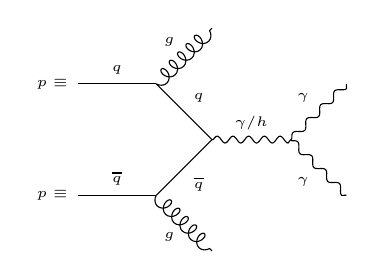
\begin{tikzpicture}
                        \begin{feynman}[small]
                            % top to bottom, pre-axion
                            \vertex (v1); % top jet vertex
                            \vertex [left=of v1] (in1) {$p \equiv$}; % top incoming particle
                            \vertex [above right=of v1] (j1) ; % top jet
                            \vertex [below right=of v1] (v3); % axion vertex
                            \vertex [below left=of v3] (v2); % bottom jet vertex
                            \vertex [below right=of v2] (j2);  % bottom jet
                            \vertex [left=of v2] (in2) {$p \equiv $};  % bottom incoming particle
                            % axion onward
                            \vertex [right=of v3] (ax);
                            \vertex [above right=of ax] (p1);
                            \vertex [below right=of ax] (p2);
                            
                            \diagram*{
                                (in1) -- [plain, edge label=$q$] (v1),
                                (in2) -- [plain, edge label=$\overline{q}$] (v2),
                                (v1) -- [gluon, edge label=$g$] (j1),
                                (v2) -- [gluon, edge label'=$g$] (j2),
                                (v1) -- [plain, edge label=$q$] (v3),
                                (v2) -- [plain, edge label'=$\overline{q}$] (v3),
                                (v3) -- [boson, edge label=$\gamma/h$] (ax),
                                (ax) -- [boson, edge label=$\gamma$] (p1),
                                (ax) -- [boson, edge label'=$\gamma$] (p2),
                            };
                        \end{feynman}
                    \end{tikzpicture}
                }
            }
        \end{column}
        
        \begin{column}{0.5\linewidth}
            \centering
            \uncover<+(1)->{
                \scalebox{0.75}{
                    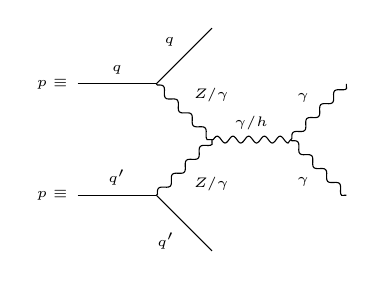
\begin{tikzpicture}
                        \begin{feynman}[small]
                            % top to bottom, pre-axion
                            \vertex (v1); % top jet vertex
                            \vertex [left=of v1] (in1) {$p \equiv$}; % top incoming particle
                            \vertex [above right=of v1] (j1) ; % top jet
                            \vertex [below right=of v1] (v3); % axion vertex
                            \vertex [below left=of v3] (v2); % bottom jet vertex
                            \vertex [below right=of v2] (j2);  % bottom jet
                            \vertex [left=of v2] (in2) {$p \equiv $};  % bottom incoming particle
                            % axion onward
                            \vertex [right=of v3] (ax);
                            \vertex [above right=of ax] (p1);
                            \vertex [below right=of ax] (p2);
                            
                            \diagram*{
                                (in1) -- [plain, edge label=$q$] (v1),
                                (in2) -- [plain, edge label=$q'$] (v2),
                                (v1) -- [plain, edge label=$q$] (j1),
                                (v2) -- [plain, edge label'=$q'$] (j2),
                                (v1) -- [boson, edge label=$Z/\gamma$] (v3),
                                (v2) -- [boson, edge label'=$Z/\gamma$] (v3),
                                (v3) -- [boson, edge label=$\gamma/h$] (ax),
                                (ax) -- [boson, edge label=$\gamma$] (p1),
                                (ax) -- [boson, edge label'=$\gamma$] (p2),
                            };
                        \end{feynman}
                    \end{tikzpicture}
                }
            }
        \end{column}
    \end{columns}
\end{frame}

% 9) MG-CUTS KINEMATICS
\begin{frame}{Kinematics with MG-Level Cuts}
    \begin{columns}
        \begin{column}{0.33\linewidth}
            \centering
            \includegraphics<+(1)->[width=0.9\linewidth]{images/no_ma_cuts_kinematics/selection_8.png} % delta eta jj
        \end{column}
        \begin{column}{0.33\linewidth}
            \centering
            \includegraphics<+(1)->[width=0.9\linewidth]{images/no_ma_cuts_kinematics/selection_7.png} % m gamma gamma
        \end{column}
        \begin{column}{0.33\linewidth}
            \centering
            \includegraphics<+(1)->[width=0.9\linewidth]{images/no_ma_cuts_kinematics/selection_9.png} % m gamma gamma
        \end{column}
    \end{columns}
    \begin{columns}
        \begin{column}{0.5\linewidth}
            \centering
            \includegraphics<+(1)->[width=0.6\linewidth]{images/no_ma_cuts_kinematics/selection_10.png} % delta eta jj
        \end{column}
        \begin{column}{0.5\linewidth}
            \centering
            \includegraphics<+(1)->[width=0.6\linewidth]{images/no_ma_cuts_kinematics/THT_stitch.png} % THT
        \end{column}
    \end{columns}
    \begin{block}<+(1)->{Comments}
        The first four kinematic plots exhibit high signal-background discriminating power in the following kinematic variables.
        
        \smallskip
        
        $\Delta \eta^{jj}, m^{jj}, m^{\gamma \gamma}, p_T^{\gamma}$
        
        \smallskip
        
        This is a little more subtle in the $\Delta \eta^{jj}$ case, but the VBF subset of our signal has higher $\Delta \eta^{jj}$ so cuts in this variable will boost significance. These plots motivate our optimization. The final kinematic plot demonstrates how our $H_T$-binned background samples are ``stiched'' together smoothly (noise occurring only at the higher end of our final $H_T$ bin).
    \end{block}
\end{frame}


%
% SEC: EVENT SELECTION CRITERIA
%
\section{Event Selection Criteria}

% 10) FIRST (JET) OPTIMIZATION
\begin{frame}{Jet Variable Selection Optimization ($\Delta \eta^{jj}$, $m^{jj}$)}
    \begin{block}<+(1)->{Process}
        We begin by optimizing the $\Delta \eta^{jj}$ and $m^{jj}$ selections simultaneously (to account for correlations). We perform a gridsearch on pairs of selections of the form $|\Delta \eta^{jj}| > \eta_0$, $m^{jj} > m^j_0$ on the following values ($m^{jj}$ given in GeV).
        
        \smallskip
        
        $(\eta_0, m^j_0) \in \{2.6, 3.1, 3.6, 4.1, 4.6, 5.1, 5.6, 6.1\} \times \{120, 500, 750, 1000, 1250, 1500, 1750, 2000\}$
        
        \smallskip
        
        We compute significance in two ways on each of these $8 \cdot 8 = 64$ scenarios: without (left) and with (right) a systematic uncertainty term. To avoid divergences arising from low background yield, we alter the base significance form $\frac{S}{B}$ to $\frac{S}{\sqrt{S + B}}$ and implement a systematic uncertainty approximation with the modification $S/\sqrt{S + B + (r \cdot B)^2}$ for $r \in [0,1]$
    \end{block}
    \begin{columns}
        \begin{column}{0.5\linewidth}
            \centering
            \includegraphics<+(1)->[width=0.6\linewidth]{images/first_optimization/heatmaps/sdeta_mjj_optimization_heatmap_r0.png} % r=0
        \end{column}
        \begin{column}{0.5\linewidth}
            \centering
            \includegraphics<+(1)->[width=0.6\linewidth]{images/first_optimization/heatmaps/sdeta_mjj_optimization_heatmap_r025.png} % r=0.25
        \end{column}
    \end{columns}
    \begin{block}<4->{Conclusions}
        Experimental constraints motivate prioritization of higher $\Delta \eta^{jj}$ cuts, and our approximation of sys. uncert. fails at higher $m^{jj}$ cuts. Thus, we invoke the non-sys. uncert. results and pursue two selection pairs: a tight (lower significance/more experimental feasibility) cut $(\eta_0, m^j_0) = (3.6, 1250)$ and a loose (higher significance/less experimental feasibility) cut $(\eta_0, m^j_0) = (2.6, 1250)$.
    \end{block}
\end{frame}

% 11) PHOTON DISCRIMINATION CHECK
\begin{frame}{Checking Photon Discriminating Power}
    \begin{block}<+(1)->{Confirmation}
        Before proceeding to the optimization for the other two variables---$m^{\gamma \gamma}, p_T^\gamma$---we quickly check that our tight/loose $\Delta \eta^{jj}, m^{jj}$ cuts haven't reduced discriminating power. We consider kinematic plots in the tight cuts scenario.
    \end{block}
    
    \bigskip
    
    \begin{columns}
        \begin{column}{0.5\linewidth}
            \centering
            \includegraphics<+(1)->[width=0.75\linewidth]{images/first_optimization/tight_kinematics/selection_9.png}
        \end{column}
        \begin{column}{0.5\linewidth}
            \centering
            \includegraphics<+(1)->[width=0.75\linewidth]{images/first_optimization/tight_kinematics/selection_10.png} % r=0
        \end{column}
    \end{columns}
    
    \bigskip
    
    
    \begin{block}<4->{Conclusions}
        Our discriminating power has been preserved (these plots behave similarly in the loose cuts scenario), allowing us to continue on to a photon kinematics optimization routine.
    \end{block}
\end{frame}

% 12) SECOND (PHOTON) OPTIMIZATION
\begin{frame}{Photon Variable Selection Optimization ($m^{\gamma \gamma}$, $p_T^{\gamma}$)}
    \begin{block}<+(1)->{Process}
        We now optimize the $m^{\gamma \gamma}$ and $p_T^{\gamma}$ selections simultaneously, performing a gridsearch on pairs of selections of the form $m^{\gamma \gamma} > m^\gamma_0$, $p_T^\gamma > \gamma_0$ on the following values (both variables given in GeV).
        
        \smallskip
        
        $(m^\gamma_0, \gamma_0) \in \{200, 250, 300, 350, 400, 450, 500, 550, 600, 650, 700\} \times \{100, 150, 200, 250, 300, 350, 400, 450, 500\}$
        
        \smallskip
        
        We compute significance in two ways on each of these $11 \cdot 9 = 99$ scenarios---in particular, using different systematic uncertainty coefficients---for both the tight (left two plots) and loose (right two plots) jet kinematic selections.
    \end{block}
    
    \smallskip
    
    \begin{columns}
        \begin{column}{0.25\linewidth}
            \centering
            \includegraphics<+(1)->[width=\linewidth]{images/second_optimization/heatmaps/tight_pta_maa_optimization_heatmap_r01.png} % r=0
        \end{column}
        \begin{column}{0.25\linewidth}
            \centering
            \includegraphics<+(1)->[width=\linewidth]{images/second_optimization/heatmaps/tight_pta_maa_optimization_heatmap_r025.png} % r=0
        \end{column}
        \begin{column}{0.25\linewidth}
            \centering
            \includegraphics<+(1)->[width=\linewidth]{images/second_optimization/heatmaps/loose_pta_maa_optimization_heatmap_r01.png} % r=0.25
        \end{column}
        \begin{column}{0.25\linewidth}
            \centering
           \includegraphics<+(1)->[width=\linewidth]{images/second_optimization/heatmaps/loose_pta_maa_optimization_heatmap_r025.png} % r=0.25
        \end{column}
    \end{columns}
    
    \smallskip
    
    \begin{block}<6->{Conclusions}
        Each heatmap provides us with a slightly different local maxima for significance: we therefore decide to pursue four $(m^\gamma_0, \gamma_0)$ selections (ordering coinciding with the heatmap ordering).
        
        \smallskip
        
        $(m^\gamma_0, \gamma_0) \in \{(400, 250), (500, 300), (350, 250), (400, 350)\}$
    \end{block}
\end{frame}

% 13) THIRD (JET) OPTIMIZATION
\begin{frame}{Jet Variable Selection Optimization, Again ($\Delta \eta^{jj}$, $m^{jj}$)}
    \begin{block}<+(1)->{Process}
        Given our four pairs of $m^{\gamma \gamma}$, $p_T^{\gamma}$ selections, we now return to the jet kinematic variables to explore significance in the $\Delta \eta^{jj}$, $m^{jj}$ phase space for each photon kinematics selection. This time, we perform a gridsearch on a smaller phase space region, with pairs of selections of the form $|\Delta \eta^{jj}| > \eta_0$, $m^{jj} > m^j_0$ on the following values ($m^{jj}$ again given in GeV).
        
        \smallskip
        
        $(\eta_1, m^j_1) \in \{2.6, 3.1, 3.6, 4.1\} \times \{750, 1000, 1250, 1500, 1750, 2000\}$
        
        \smallskip
        
        We compute significance in just one way on each of these $4 \cdot 6 = 24$ scenarios, simply using the systematic uncertainty coefficient which led to the selection of that particular $m^{\gamma \gamma}$, $p_T^{\gamma}$ selections. Our plots are then ordered as follows.
        
        \smallskip
        
        $(m^\gamma_0, \gamma_0) = (400, 250), (m^\gamma_0, \gamma_0) = (500, 300), (m^\gamma_0, \gamma_0) = (350, 250), (m^\gamma_0, \gamma_0) = (400, 350)$
    \end{block}
    
    \smallskip
    
    \begin{columns}
        \begin{column}{0.25\linewidth}
            \centering
            \includegraphics<+(1)->[width=\linewidth]{images/third_optimization/heatmaps/maa400_pta250sdeta_mjj_optimization_heatmap_r01.png}
        \end{column}
        \begin{column}{0.25\linewidth}
            \centering
            \includegraphics<+(1)->[width=\linewidth]{images/third_optimization/heatmaps/maa500_pta300sdeta_mjj_optimization_heatmap_r025.png}
        \end{column}
        \begin{column}{0.25\linewidth}
            \centering
            \includegraphics<+(1)->[width=\linewidth]{images/third_optimization/heatmaps/maa350_pta250sdeta_mjj_optimization_heatmap_r01.png}
        \end{column}
        \begin{column}{0.25\linewidth}
            \centering
            \includegraphics<+(1)->[width=\linewidth]{images/third_optimization/heatmaps/maa400_pta350sdeta_mjj_optimization_heatmap_r025.png}
        \end{column}
    \end{columns}
    
    \begin{block}<6->{Conclusions}
        Our four scenarios exhibit an approximately uniform shape, with a maximum near $(\eta_1, m^j_1) = (2.6, 750)$. Once again, we consider high $\Delta \eta^{jj}$ selections to be more experimentally feasible. We also seek to incorporate a realistically high systematic uncertainty. These priorities motivate the following selections.
        
        \smallskip
        
        $|\Delta \eta^{jj}| > 3.6, m^{jj} > 750, m^{\gamma \gamma} > 500, p_T^\gamma > 300$
    \end{block}
\end{frame}

% 14) SELECTION SIGNIFICANCE
\begin{frame}{Selection Significance}
    \begin{columns}
        \begin{column}{0.45\linewidth}
            \begin{block}<+(1)->{Objective}
                Given our new parameter selections, want to quickly summarize our progress.
                \begin{itemize}
                    \item Want to compare signal-background kinematic plots normalized to cross section between before (below) and after (right, top) selections are made
                    \item Want to examine how significance scales with luminosity for different significance metrics (right, bottom)
                \end{itemize}
            \end{block}
            
            \bigskip
            
            \centering
            \includegraphics<+(1)->[width=0.8\linewidth]{images/pre_post_stacked_comparison/pre_selection_7.png}
        \end{column}
        \begin{column}{0.45\linewidth}
            \centering
            \includegraphics<+(1)->[width=0.8\linewidth]{images/pre_post_stacked_comparison/post_selection_7.png}
            \includegraphics<+(1)->[width=0.8\linewidth]{images/third_optimization/second_lum_comparison_plot.png}
            
            \smallskip
            
            \begin{block}<5->{Conclusions}
                We've selected a region of phase space where our new physics processes dominate and discovery potential is high.
            \end{block}
        \end{column}
    \end{columns}
\end{frame}

%
% SEC: FINAL THOUGHTS
%
\section{Final Thoughts}

% 15) FINAL THOUGHTS
\begin{frame}[label=current]{Final Thoughts}
    \begin{block}<+(1)->{Summary}
        \begin{itemize}
            \item Introduced the theory of our particular BSM interest---the axion---and the collider topology we plan to use to study it, vector boson fusion (VBF)
            \item Discussed our generation of signal events, including imposed MadGraph-level selections to increase VBF purity
            \item Examined our generation of background events, including the choice of two distinct background channels and our $H_T$ binning process
            \item Analyzed kinematic variables and elaborated on our three-step selection optimization process on $\Delta \eta^{jj}, m^{jj}, m^{\gamma \gamma}, p_T^j$, eventually arriving at an experimentally and statistically motivated selection for each of these variable
            \item Investigated signal versus background yield and the significance associated with our four final selections
        \end{itemize}
    \end{block}
    
    \bigskip
    
    \begin{block}<+(1)->{Next Steps}
            \begin{itemize}
                \item Resolve technical issues (potentially relating to \texttt{ax > a a} decay) and study how our findings vary with axions of different masses
                \item Investigate why virtual axion processes dominate (thoughts?)
                \item Anything else?
            \end{itemize}
    \end{block}
\end{frame}

\end{document}